\section{Pianificazione}
Lo sviluppo del progetto è suddiviso nelle seguenti fasi:
    \begin{itemize}
        \item  RTB
        \item PB
    \end{itemize}
    \subsection{RTB}
    Nel periodo dal 04/11/2024 al 17/01/2025 verranno prodotti i seguenti documenti:
        \begin{itemize}
            \item "Norme di progetto"
            \item "Piano di progetto"
            \item "Analisi dei requisiti"
            \item "Piano di qualifica"
            \item "Glossario"
        \end{itemize}
    Inoltre verrà realizzato il Proof of Concept, per valutare la fattibilità tecnologica del progetto.
        \subsubsection{Sprint 1 (dal 11/11/2024 al 22/11/2024)}
        In questo periodo verrà definito il way of working, documentato nelle
        "Norme di progetto". Per quanto riguarda la gestione di progetto, verranno 
        pianificate le attività, stilato un preventivo e analizzati i rischi che potrebbero
        incidere sullo svolgimento del progetto. Infine si comincerà a redigere il 
        "Glossario", fondamentale per garantire una chiara comprensione e comunicazione all'
        interno del team e con il proponente.
        \\
        \begin{figure}[h!]
            \centering
            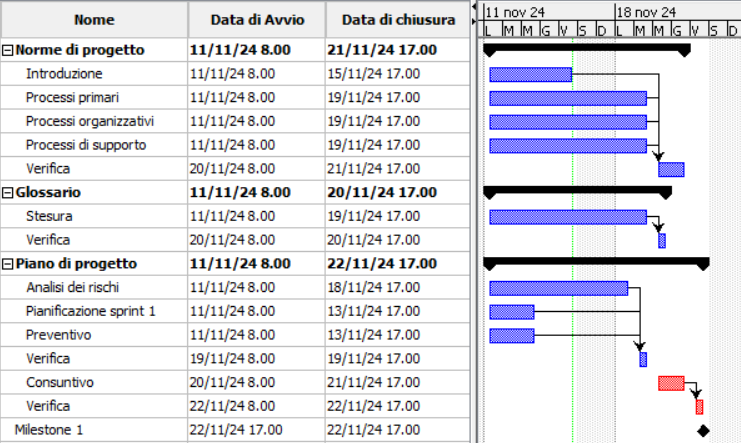
\includegraphics[scale = 0.85]{template/images/gantt1.png}
            \caption{Diagramma di Gantt sprint 1}
            \label{fig:3.1} % Etichetta per il riferimento
        \end{figure}
        